% Load the kaohandt class (with the default options)
\documentclass[
	a4paper,
	fontsize=10pt, % Base font size
	twoside=false, % If true, use different layouts for even and odd pages (in particular, if twoside=true, the margin column will be always on the outside)
	secnumdepth=2, % How deep to number headings. Defaults to 2 (subsections)
	%abstract=true, % Uncomment to print the title of the abstract
]{kaohandt}

% Choose the language
\usepackage[english]{babel} % Load characters and hyphenation
\usepackage[english=british]{csquotes}	% English quotes

% Load packages for testing
\usepackage{blindtext}
%\usepackage{showframe} % Uncomment to show boxes around the text area, margin, header and footer
%\usepackage{showlabels} % Uncomment to output the content of \label commands to the document where they are used

\graphicspath{{../img/}{./}} % Paths where images are looked for

% Load mathematical packages for theorems and related environments.
\usepackage{kaotheorems}

% Load the bibliography package
\usepackage{kaobiblio}
\addbibresource{report-template.bib} % Bibliography file

% Load the package for hyperreferences
\usepackage{kaorefs}

% Load the package for tabularx
\usepackage{tabularx}

%----------------------------------------------------------------------------------------

\begin{document}

%----------------------------------------------------------------------------------------
%	REPORT INFORMATION
%----------------------------------------------------------------------------------------

\title[]{Sommelier:\\ A personal wine recommendation engine\sidenote{Project step III updated.}}
\subtitle{ANLY-605 (Fall 2022) at Georgetown University}

\author[JG, EL, RQ]{Jingsong Gao\thanks{\href{mailto:jg2109@georgetown.edu}{jg2109@georgetown.edu}}\\
Ercong Luo \thanks{\href{mailto:el890@georgetown.edu}{el890@georgetown.edu}}\\
Rui Qiu \thanks{\href{mailto:rq47@georgetown.edu}{rq47@georgetown.edu}}}

\date{\today}

%----------------------------------------------------------------------------------------
%	TITLE AND ABSTRACT
%----------------------------------------------------------------------------------------

\maketitle
\newpage
\tableofcontents
\listoffigures % Output the list of figures
\listoftables % Output the list of tables
\newpage
% \margintoc


% \begin{abstract}
% \noindent
% \blindtext
% \end{abstract}

% {\noindent\textbf{Keywords:} \LaTeX, Kao, handout, article, report}

\medskip

%----------------------------------------------------------------------------------------
%	MAIN BODY
%----------------------------------------------------------------------------------------

\section{Project Description}

\subsection{General Description}

With our app Sommelier, an end user can find recommendations of wine region and grape varietals based on a few keywords of flavor notes. This saves them the time, money and liver to try many bottles of wine that they don’t like.

\subsection{Project Deliveries}

An interactive web application where the end user inputs a description of their wine preference, and the application surfaces a list of top 5 recommendations of \texttt{<wine region, grape variety>} pairs. The back-end of the application is where natural language processing and machine learning algorithms are deployed to surface recommendations at the highest accuracy possible.

\subsection{Out of Scope}

This project will not include any background educational knowledge on wine tasting. Nor will the application have any mechanisms for collecting user feedback in the first release.

\subsection{Assumptions}

We assume that:

\begin{enumerate}
	\item The expert wine reviews in the training dataset are unbiased and accurate descriptions of wine flavors.
	\item The primary factors that influence the flavor of a wine are the region of production and the grape varietal, hence the choice of surfacing \texttt{<wine region, grape variety>} pairs as recommendations to an end user.
\end{enumerate}

\subsection{Constraints}

For the constraints, we have:

\begin{itemize}
	\item \textbf{Biased Review:} The reviews we will use to train the classifier, especially, the description of notes, are subjective. The reviewers are also anonymous. Amateur and professional tasters might use different words to describe the same wine.
	\item \textbf{Outdated Wine Data:} The wine dataset is updated on November 22nd, 2017, so any wines produced after the date will not be recommended.
	\item \textbf{Incompatible Target:} The classification model is trained to provide a tuple \texttt{<wine region, grape variety>} that matches the description of a review. But since recommendation to users is an open-ended question, it will be difficult to evaluate the “goodness” of recommendations until there is enough collected user feedback for product analysis and review.
	\item \textbf{Limited Computing Resource:} Cloud service providers have limited computing resources for free deployment, especially the RAM:
		\begin{itemize}
			\item For Heroku, the free Dyno has 512MB RAM.
			\item For AWS EC2, the low-end t4g.nano instance (0.0042 USD/h) also has 512MB RAM.
		\end{itemize}
		Considering the server handler to process requests and other resources need to be loaded into the memory, models have to be smaller than 200 megabytes altogether. This could prevent us from using most deep learning-based solutions.
	\item \textbf{Discrepancy Between Descriptions and Reviews:} We will use text-based reviews as proxies for a user’s description of their wine preference. Admittedly, this will now account for the variance in user input in terms of word choice preference, sentence lengths, and subjective bias that cannot be captured by our language model.
\end{itemize}

\subsection{Development Roadmap}

Because most NLP models today are based on transformers, and our early thought for this project is that a transformer-based model is going to outperform a traditional model like SVM or tree-based ensemble learning. That being said, we still followed class requirements and trained models such as an SVM, a perceptron, and a naive Bayes classifier from sklearn and constructed a stacked model. We included evaluations for both the transformer model (BERT-mini) and the stacked ensemble model.

Items in bold are listed as course-required stages, while the ones in italic are extra milestones.

\begin{itemize}
	\item \textbf{Stage 1: Problem Identification and project charter. Submitted by Sept 7, 2022.}
		\begin{itemize}
			\item Create a repository for the project and set up the developing environment. Done by Sept 14, 2022.
			\item Initial training of the candidate model “Wine BERT”. Done by Sept 21, 2022.
		\end{itemize}
	\item \textbf{Stage 2: Solution by generative method (this report). Submitted by Sept 28, 2022.}
		\begin{itemize}
			\item Model performance comparison: Wine BERT vs generative methods (included in the report). Submitted by Sept 28, 2022.
		\end{itemize}
	\item \textbf{Stage 3: Initial deployment. Submit by Oct 12, 2022.}
	\item \textbf{Stage 4: Solution by hyperparameter optimization. Submit by Oct 26, 2022.}
	\item \textbf{Stage 5: Complete project. Submit by Nov 16, 2022.}
\end{itemize}

\section{Introduction}

Whenever we talk to a wine connoisseur, we will hear them talk about their wine preferences based on two primary factors: the region where the wine is from and the grape varietal from which the wine is made. It is obviously a steep learning curve for a newcomer to know their personal wine preferences in terms of these two primary factors because it requires trial and error that most of us don’t have the money, time or the liver to do. But what if we have our personal digital wine steward, or a sommelier as the French call it? That is what our app is for.

Sommelier App takes advantage of natural language processing and machine learning algorithms, trained using a dataset of 117283 wine reviews written by expert wine tasters to learn the differences in described flavor notes that differentiate a dataset of over 500 \texttt{<region, grape varietal>} pairs.

\section{Analysis of the Dataset of Trained Model}

\subsection{Exploratory Analysis}

Since our dataset is text-based, the exploratory data analysis (EDA) procedure is rather limited. A typical sample of data is listed in Table~\ref{tab:raw_samples}. \\

\begin{table}[ht]
	\begin{tabular}{lll} \toprule
		\tiny\texttt{} & \tiny\texttt{Description} & \tiny\texttt{region\_variety}  \\ \midrule
		\tiny\texttt{0} & \tiny\texttt{The deep red-black color reaches...} & \tiny\texttt{France-Languedoc-Roussillon:Cabernet Sauvignon}  \\
		\tiny\texttt{1} & \tiny\texttt{Complexity and varietal character...} & \tiny\texttt{US-California:Merlot} \\
		\tiny\texttt{2} & \tiny\texttt{Rhubarb and cranberry fruit, along...} & \tiny\texttt{US-Oregon:Pinot Noir} \\ \bottomrule
	\end{tabular}
	\caption{Two samples in raw data.}
	\label{tab:raw_samples}
\end{table}

After preprocessing, the sample data we use to train the model are listed in Table~\ref{tab:processed_samples}. \\

\begin{table}[ht]
	\begin{tabular}{lll} \toprule
		\tiny\texttt{} & \tiny\texttt{keywords} & \tiny\texttt{region\_variety}  \\ \midrule
		\tiny\texttt{0} & \tiny\texttt{core adequate acidity moderate...} & \tiny\texttt{265}  \\
		\tiny\texttt{1} & \tiny\texttt{complexity varietal character black plum...} & \tiny\texttt{17} \\
		\tiny\texttt{2} & \tiny\texttt{rhubarb cranberry fruit red apple light simple...} & \tiny\texttt{4} \\
		\tiny\texttt{3} & \tiny\texttt{impressive fullness ripeness black cherry leat...} & \tiny\texttt{251} \\
		\tiny\texttt{4} & \tiny\texttt{dusty tones mineral saffron pollen concentrate...} & \tiny\texttt{11} \\ \bottomrule
	\end{tabular}\\
	\caption{Five pre-processed samples. \emph{(Descriptive keywords are extracted from raw reviews, region\_variety pairs are converted to numeric labels)}}
	\label{tab:processed_samples}
\end{table}

There are in total 584 region varieties in the dataset. A slim version of 11680 records are included as the training set of all candidate models below.

The keywords are vectorized into a feature vector of length 6081, and a slice of descriptive features used in wine reviews are: \\

\texttt{Vectorizer features: ['bell', 'bellangelo', 'belzbrunnen', 'benito', 'benjamin', 'berenguer', 'beresan', 'bergamot', 'bergerac', 'bernard', 'berried', 'berries', 'berry', 'berryish', 'berrylicious', 'bertani', 'best', 'better', 'betz', 'beverage', 'bianca', 'bianco', 'biancolella', 'bical', 'bieler', 'bienenberg', 'big', 'bigger', 'biggest', 'bigtime', 'bilberry', 'bill', 'billards', 'billing', 'billo', 'bing', 'biodynamic', 'biodynamically', 'birch', 'bird', 'birds', 'biscotti', 'biscuit', 'biscuits', 'biscuity', 'bisquertt', 'bistro', 'bite', 'bites', 'biting', 'bitner', 'bits', 'bitter', 'bitterness', 'bitters', 'bittersweet', 'black', 'blackberries', 'blackberrry', 'blackberry', 'blackcurrant', 'blackened', 'blackness', 'blacktop', 'blanc', 'blanca', 'blanched', 'blanco', 'blancs', 'bland', 'blangé', 'blasting', 'blatant', 'blaufränkisch', 'blaye', 'blazing', 'blend', 'blended', 'blending', 'blends', 'bleue', 'blind', 'bliss', 'blockbuster', 'blockier', 'blocks', 'blocky', 'blood', 'bloody', 'bloom', 'blossom', 'blossoms', 'blossomy', 'blowsy', 'blue', 'blueberries', 'blueberry', 'bluebery', 'blush', 'board']}

\subsection{Baseline Model: BERT-mini}

Our baseline model is a little bit “unorthodox”. We use the \href{https://huggingface.co/google/bert_uncased_L-4_H-256_A-4}{BERT-mini} model with the raw review texts as inputs. There are several reasons for this:

\begin{itemize}
	\item \textbf{Pre-knowledge} \\
	BERT models are pre-trained on a large corpus of multi-domain text and learned a lot of general language knowledge. We only need to fine-tune the model by training it with a much smaller dataset specific to our task.
	\item \textbf{Powerful Text Tokenizer} \\
	BERT models have a strong text tokenizer with a vocabulary of 30k words and a word-piece strategy to handle out-of-vocabulary words. This means we don’t need to do any preprocessing (such as punctuation cleaning, keywords extraction, etc.) on our text data.
	\item \textbf{Low Computing Cost} \\
	BERT series are very large models and require a lot of computing resources (CPU, memory, GPU). We use a mini version of BERT that is only 50MB in size and is able to run relatively fast with limited computing resources.
\end{itemize}

On a single GPU, it took 35 minutes to finetune BERT-mini on the full training data and 7 seconds to evaluate the model on the full test data. The top-5 accuracy is 92.0\% on the training data and 83.4\% on the test data.

\subsection{Metric: Top-5 Accuracy}

In classification tasks, we usually use \textbf{accuracy} (or top-1 accuracy) as a metric for model evaluation. An evaluation is considered accurate only when the model prediction and the true label are identical.

By \textbf{top-5 accuracy}, we meet that an evaluation is considered accurate if the correct label is within the top-5 predictions by posterior probability. So a 92.0\% accuracy in our case means that 92.0\% of the time, the correct label is within the top-5 predictions on a given input. This top-5 accuracy metric is chosen because:

\begin{itemize}
	\item \textbf{Similarity between wines} \\
	When a user types in a description of a wine, the model should be able to return a list of top-5 recommended wines. The user can then choose the one that best matches his/her taste.
	\item \textbf{Generalization of the model} \\
	By using a relatively lenient top-5 accuracy, we gave the model more space and tolerance to learn the similarities between wines. The model was taught to understand a one-to-many relationship from reviews to wines, rather than the strict one-to-one relationship when using the top-1 accuracy.
	\item \textbf{Alignment with usage scenarios} \\
	The usage scenario of our application is to recommend the top-5 relevant wines to users according to their descriptions. Using top-5 accuracy helps the model to be consistent during training and inference.
\end{itemize}

\section{Model Selection}

\subsection{Individual Models and Stacked Model}

Since we are selecting candidate models for stacking, and ultimately competing with BERT-mini, we have decided to start from basic classification models ranging from Multinomial Naïve Bayes, Perceptron, Linear Support Vector Machine Classifier, Decision Tree Classifier, and Logistic Regression Classifier as our candidates.

Figure~\ref{fig:acc_test} demonstrates the classification accuracy (top-5 accuracy) on the testing set, and we can see that Logistic Regression, Naive Bayes, and Linear SVM are 3 top candidates. Don’t be fooled by the accuracy barely past 0.5, it’s already pretty impressive considering the problem we are tackling is to find the top 5 recommendations from over 500 wines that fit a verbal description. And this is achieved even without hyperparameter tuning.

The strategy and sequence we used to find the right candidates can be summarized in two sentences:

\begin{enumerate}
	\item Level 0 models should be ordered from best to worst in terms of performance. An analog is to use stepwise linear model selection from a null model. Specifically, we add the model with the best performance, then the second best to see if it improves, etc.
	\item Level 1 models (meta learner) don’t need to be complex models. Given that level 0 models are already powerful models, the meta learner is simply utilized for aggregating and calibrating predictions from the base learner.
\end{enumerate}

We also would like to recycle the Logistic Regression Classifier as a level 1 model (meta learner) to aggregate the results of the level 0 models.

We trained two combinations of stacked model following the naming convention below:

\begin{itemize}
	\item We use the initials of the level 0 candidates, and stitch them together in a sequential order. Then we connect the letters with the initial of the level 1 model using an underscore.
	\item In this manner, we have \texttt{stacked\_ln\_l} stands for a stacking classifier with a logistic regression classifier + a naïve Bayes classifier as level 0, and a logistic classifier as level 1.
	\item And \texttt{stacked\_ls\_l}, a stacking classifier with a logistic regression + a linear SVM as level 0, and a logistic classifier (again) as level 1.
\end{itemize}

\begin{figure}[h]
	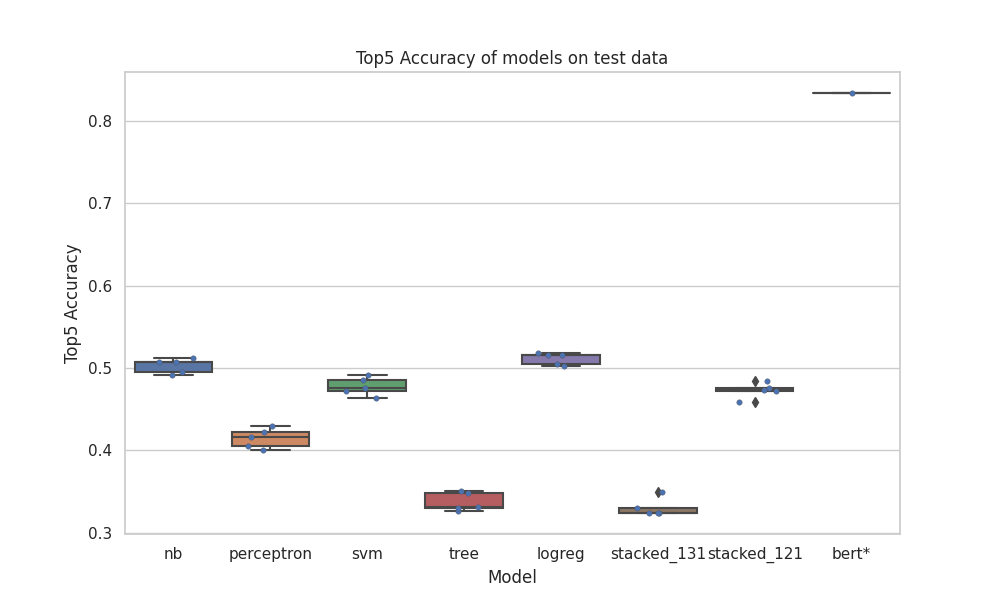
\includegraphics{metric_test_score}
	\caption{Top5 Accuracy for models on test data. \emph{Note: BERT model only has one data point as cross-validation was not performed.}}
	\label{fig:acc_test}
\end{figure}

We ruled out the ensemble models in stacking, since the training time of ensemble models in our case is comparatively long due to the size and feature number of the dataset.

\subsection{Model Performance Evaluation}

From the previous boxplot, we learned that the stacking method did not take the model performance to the next level. The performance of BERT-mini is still far better.

\begin{figure}[h]
	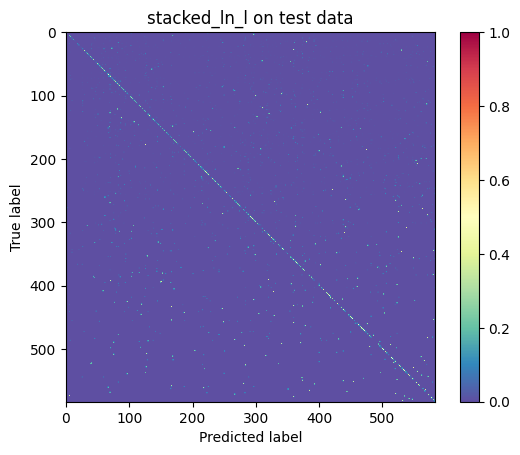
\includegraphics[width=0.49\textwidth]{confusion_matrix_stacked_ln_l_test}
	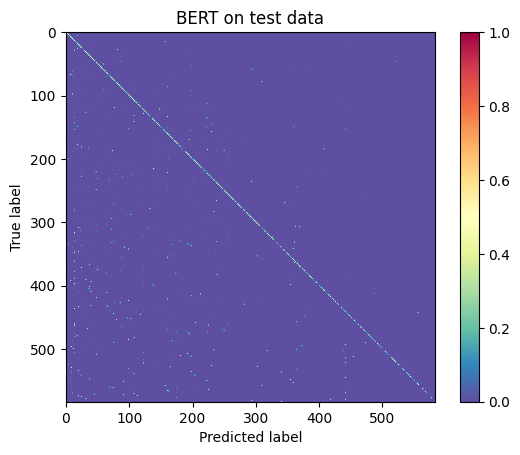
\includegraphics[width=0.49\textwidth]{confusion_matrix_bert_test}
	\caption{Confusion matrix of the stacked model \texttt{stacked\_ln\_l} and BERT-mini on test data.}
	\label{fig:conf_mat}
\end{figure}

If we compare the confusion matrices of \texttt{stacked\_ln\_l} versus BERT-mini side-by-side (Figure~\ref{fig:conf_mat}), the BERT-mini has brighter-colored pixels concentrating on the diagonal line.

Note that both diagonal lines seem to be in greenish-blue color, however, the actual values are close to 0.5 (stacked model) and 1 (BERT-mini) respectively. This is caused by \href{https://matplotlib.org/stable/gallery/images_contours_and_fields/interpolation_methods.html}{the interpolation method for \texttt{imshow}}. Basically, the color values of each pixel are averaged to its neighbors because the original heatmap is too big to display on a small figure.

Another takeaway from the confusion matrices is that BERT-mini has a tendency to predict the response to be within class 0 and class 200. However, this is more like a coincidence as the numeric value in class is nothing but an index, which is not ordinal.


Bear in mind that we haven’t done any hyperparameter tuning in either stacked model or BERT, plus the performances in training dataset imply the existence of potential overfitting.

\subsection{Cost Estimation}

The last two aspects we would like to investigate are the fit time (Figure~\ref{fig:fit_time}) and score time (Figure~\ref{fig:score_time}), which are used to imitate the runtime of training and actual prediction.

\begin{figure}[h]
	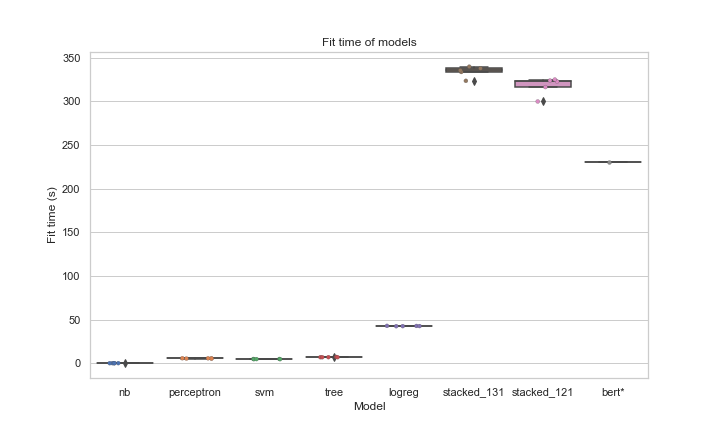
\includegraphics[]{metric_fit_time.png}
	\caption{Fit time(s) for models on training data. \emph{Note: the fit time for BERT model is estimated proportional as it was trained on the full training data.}}
	\label{fig:fit_time}
\end{figure}

Surprisingly, BERT-mini does not top the fit time in our test run. Of course, the five basic candidates are fast, and we have to admit that the logistic regression classifier is not bad in performance as well. Even though we managed to control the complexity of those two stacked models, they generally took more time to train and gave out unreliable predictions.

In practice, when we set a periodic batch job scheduled, say it’s designed to train the model with new data, the more time we need to train the model, the higher computation resources we need to fulfill such a task. And this can be translated into higher cost for the company.

\begin{figure}[h]
	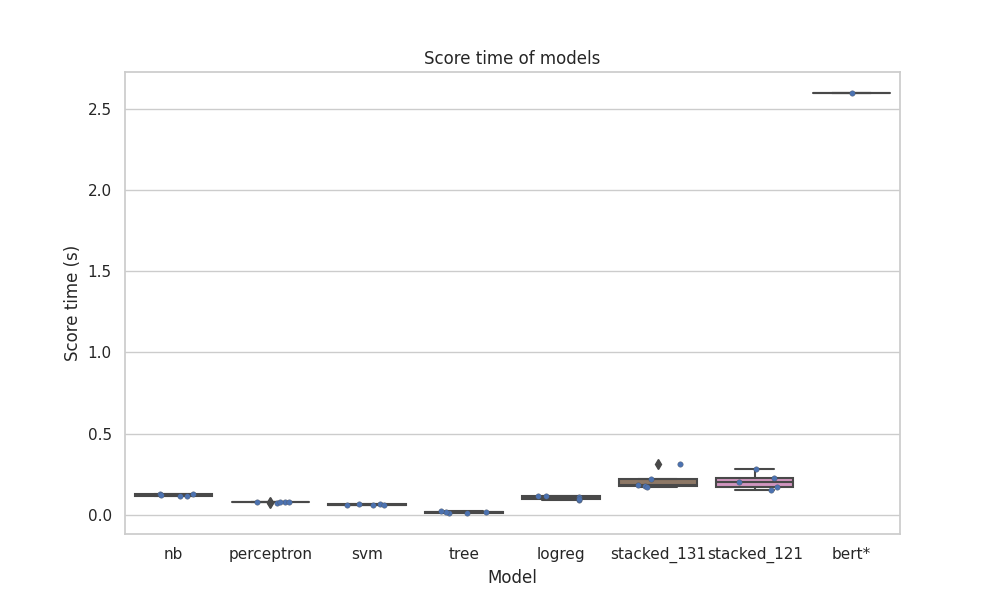
\includegraphics[]{metric_score_time.png}
	\caption{Score time(s) for models on validation data. \emph{Note: the score time for BERT model is estimated proportional as it was evaluated on the full validation data.}}
	\label{fig:score_time}
\end{figure}


BERT-mini falls to the bottom of the league in terms of score time competition. The score time in production can be translated into waiting time for the end user. But 2.5 seconds response time in frontend is not the end of the world, and hopefully this could be potentially compensated by some web page optimization tricks. Nevertheless, we should be aware of the risk of large amounts of concurrent requests in an imaginary scenario. Making the application a real-time experience is a key optimization goal for our project.

\section{Initial Deployment}

\subsection{Overview}

Dark mode support.

\begin{figure}[h]
	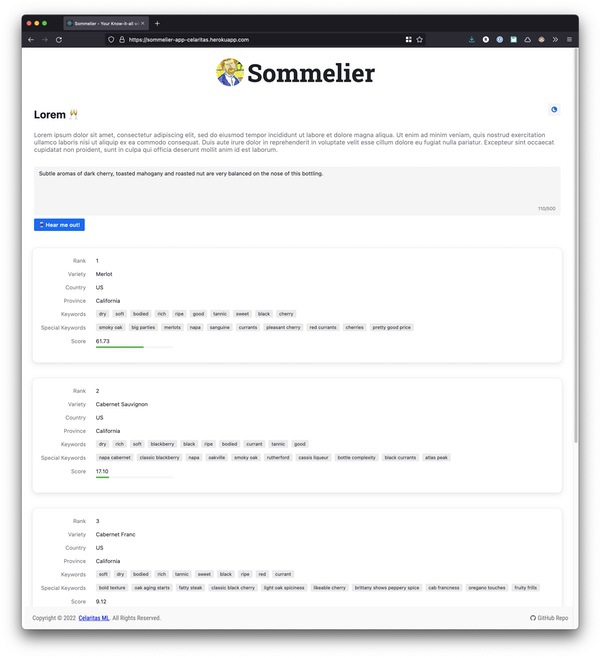
\includegraphics[width=0.49\textwidth]{sommelier-view-01.jpg}
	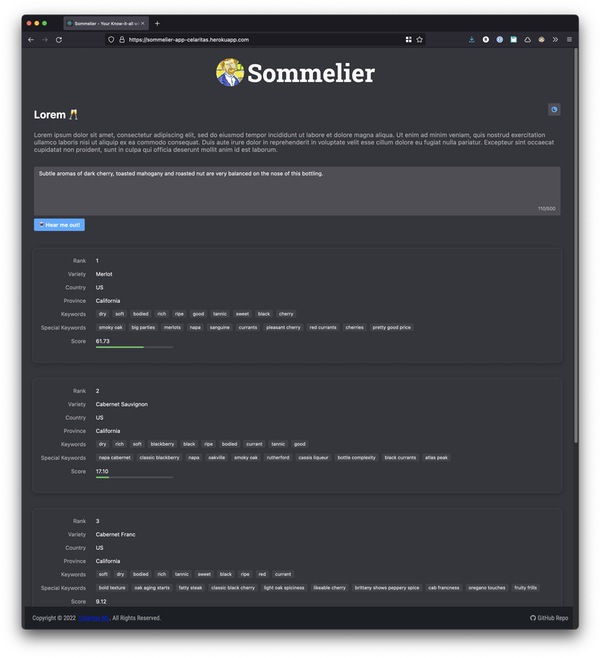
\includegraphics[width=0.49\textwidth]{sommelier-view-02.jpg}
	\caption{Snapshot of app webpage. \emph{Dark mode supported.}}
	\label{fig:app_overview}
\end{figure}

Mobile, responsive design.

\subsection{Input box and Recommendation Cards}

\begin{figure}[h]
	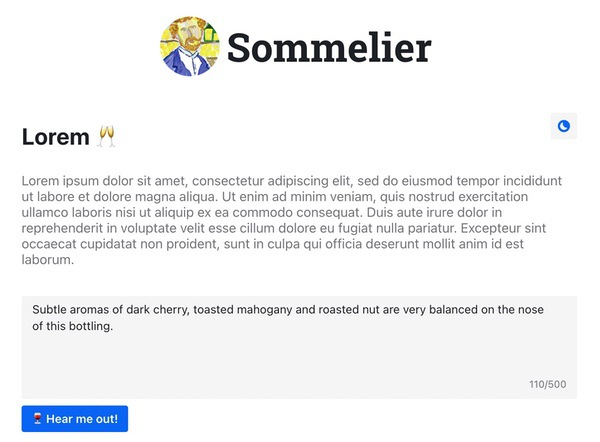
\includegraphics[]{sommelier-view-03.jpg}
	\caption{The header and an input box. \emph{Note: the prologue is placehold by lipsum.}}
	\label{fig:app_input}
\end{figure}

\begin{figure}[h]
	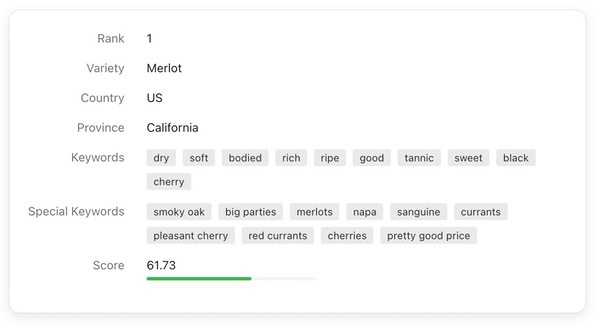
\includegraphics[]{sommelier-view-04.jpg}
	\caption{A recommendation card.}
	\label{fig:app_rec_card}
\end{figure}

\subsection{Heroku Application}

\subsubsection*{The Platform, and the Repository}

GitHub repository \href{https://github.com/CeleritasML/sommelier-app}{https://github.com/CeleritasML/sommelier-app} under the organization \href{https://github.com/CeleritasML}{CeleritasML}.

\subsubsection*{Application Path}

\href{https://sommelier-app-celaritas.herokuapp.com/}{https://sommelier-app-celaritas.herokuapp.com/}

\subsubsection*{Deployment, debugging, and updates}

Write here your introduction,\sidecite{James2013} and make sure to
reference your sources.

\blindtext\sidenote[][]{\blindtext}

\appendix % From here onwards, chapters are numbered with letters, as is the appendix convention

\section{Appendix A: Appendix Title}

\blindtext

%----------------------------------------------------------------------------------------
%	BIBLIOGRAPHY
%----------------------------------------------------------------------------------------

% The bibliography needs to be compiled with biber using your LaTeX editor, or on the command line with 'biber main' from the template directory

% \printbibliography[title=Bibliography] % Set the title of the bibliography and print the references

\end{document}
